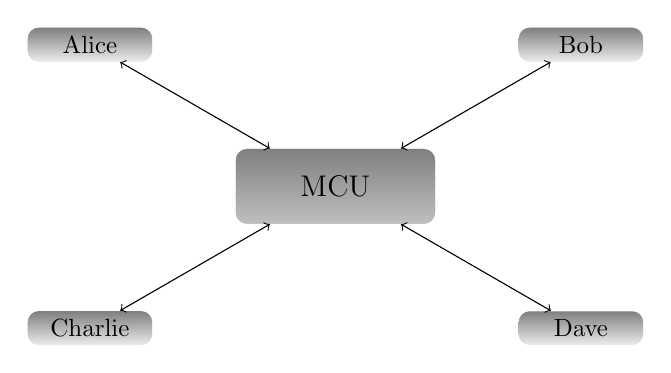
\begin{tikzpicture}[scale=.9,transform shape]
  \onslide<+->{
    \node[rectangle, fill=gray!60, bottom color=gray!50, minimum width=80pt, minimum height= 30pt] (mcu) at (0, 0) {\large MCU};
  }

  \onslide<+->{
    \tikzstyle{every node} = [rectangle, rounded corners, fill=gray!20, bottom color=gray!15, minimum width=50pt]
    \node (a) at (150: 4) {Alice};
    \node (b) at +(30: 4) {Bob};
    \node (c) at +(210: 4) {Charlie};
    \node (d) at +(330: 4) {Dave};
  }

  \onslide<+->{
    \foreach \from/\to in {a/mcu, b/mcu, c/mcu, d/mcu}
      \draw [<->] (\from) -- (\to);
  }
\end{tikzpicture}
